La comprensión actual de las neuronas artificiales, fundamentales en las redes neuronales del aprendizaje automático, se origina en la inspiración biológica y en modelos iniciales como los de Warren McCulloch, Walter Pitts y Frank Rosenblat . 

\begin{figure}[h!]
	\centering
	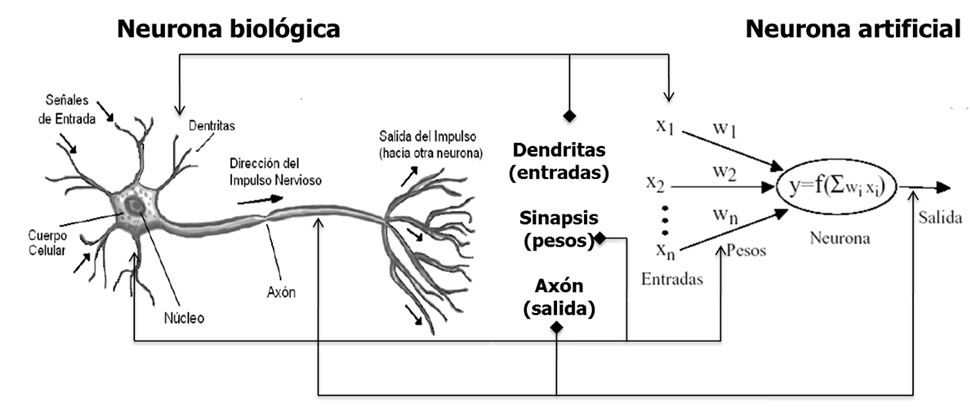
\includegraphics[width=0.65\textwidth]{capitulo2/figuras/an5.png}
	\caption{Comparación entre una neurona biológica y  artificial}
	\floatfoot{Fuente: Procedimiento para el pronóstico de la demanda mediante redes
		neuronales artificiales \cite[p. 4]{lao2017procedimiento}}
	\label{fig:an5}

\end{figure}


El enfoque de McCulloch y Pitts representaba la neurona más  o menos como una compuerta lógica, la representación actual de la neurona en el contexto de las redes neuronales muestra una mayor complejidad y una aproximación más fiel a las funciones y comportamientos observados en el enfoque propuesto por Frank Rosenblatt. Este avance refleja un modelo más detallado y más cercano a la naturaleza multifacética y dinámica de las neuronas biológicas ver Figura \ref{fig:an5}.


Estructura Básica:
\begin{itemize}
	\item	 Neurona biológica: En el cerebro humano, las neuronas son células especializadas que forman la unidad básica del sistema nervioso. Tienen una estructura celular con un cuerpo celular, dendritas, axones y sinapsis.
	\item	Neurona artificial: En informática, una neurona artificial es la unidad básica de una red neuronal. Consiste en entradas, pesos, una función de activación y una salida.
\end{itemize}


Recepción y Transmisión de Señales:
\begin{itemize}
	\item	 Neurona biológica: Las dendritas reciben señales de otras neuronas a través de sinapsis. Cuando se acumula una cantidad suficiente de señales excitatorias o inhibitorias, se genera un impulso eléctrico a lo largo del axón hasta llegar a los botones sinápticos y posteriormente a la siguiente o siguientes neuronas, donde el proceso se repite nuevamente.
	\item	Neurona artificial: Recibe múltiples entradas que son multiplicadas por su respectivo peso, el peso que interviene en las entradas será lo suficientemente grande o pequeño para influir o no en la salida que posteriormente se modificará por alguna función de activación, debido a esta tarea es que la función de sinapsis de una neurona biológica es conceptualmente equivalente a la función de los pesos en una neurona artificial. 
\end{itemize}
Adaptabilidad y Aprendizaje:
\begin{itemize}
	\item	 Neurona biológica: Las neuronas biológicas pueden cambiar su conectividad y fuerza sináptica a lo largo del tiempo, lo que permite el aprendizaje y la adaptabilidad.
	\item	Neurona artificial: Los pesos en las neuronas artificiales pueden ajustarse durante el entrenamiento mediante algoritmos de aprendizaje, lo que permite que la red neuronal aprenda y mejore su capacidad para resolver tareas específicas.
\end{itemize}

